\documentclass[12pt]{article}

\usepackage{amssymb,amsmath,amsthm}
\usepackage{graphicx}
\usepackage{pgfplotstable,booktabs,longtable}
\usepackage{float} % Package for including figures
%\usepackage{psfrag,color}

\title{Homework 7 \protect \\(Math/CS 471)}

\author{Elijah Perez \protect \newline \\ Natalie Chang}


\date{\vfill 12/13/2020}   



\begin{document}
	\maketitle
	\pagebreak
	
	\section{Introduction}
     In this report we will explore the speed up and efficiency of parallel computing when applied to numerical methods for partial differential equations. We will use the Method of Lines to calculate the numerical solution of the partial differential equation. MPI(Message Passing Interface) is the interface that will be used to make the code parallel. MPI uses distributed memory where processors have their own local memory. This is advantageous because in distributed memory systems, memory is scalable with the number of processors. The runtime of the parallel code will be compared to the runtime of serial code. It is expected that the parallel code will have an advantage in efficiency when compared to the serial code. We will be using the supercomputer Stampede2 to perform our analysis.  
	
	\section{Initial Boundary Value Problem}
	To explore the error of the numerical method and the runtime of parallel vs. serial code, we first choose a problem with a well known solution. This allows us to measure the error by directly finding the difference between our solution found using the Method of Lines and the true solution found analytically.
	\newline \newline
	The general form of the initial-boundary value problem(IBVP) being tested is:
	\newline
	\begin{center}
		$u_{tt}-[(a(x,y)u_x)_x+(a(x,y)u_y)_y]=f(x,y;t)$,\hspace{2mm} $(x,y)\in D$, \hspace{2mm}$t\in [0,T]$ \newline 
		 $u(x,y;0)=f_1(x,y), \hspace{2mm} u_t(x,y;0)=f_2(x,y)$ \newline
		$u(x,y;t)=g(x,y;t), \hspace{2mm} (x,y)\in \partial D$
	\end{center}
	
	Picking a manufactured solution allows us to find a $u(x,y;t)$ that solves this IBVP. The manufactured solution has the form: 
	\newline
		\hspace*{1in}$u(x,y;t)=sin(\omega t-k_xx)sin(k_yy),$
		\newline
		\hspace*{1in}$f(x,y;t)=u_{tt}-(a(x,y)u_x)_x-(a(x,y)u_x)_x$
		\newline
		\hspace*{1in}$f_1(x,y)=-sin(k_xx)sin(k_yy),$
		\newline
		\hspace*{1in}$f_2(x,y)=\omega cos(k_xx)sin(k_yy),$
		\newline
		\hspace*{1in}$g(x,y;t)=sin(\omega t-k_xx)sin(k_yy)$
	\newline \newline
	This allows us to select the constants $\omega$, $k_x$, and $k_y$ which will create a solution to the IBVP. We then choose a function for the wave speed $a(x,y)$. Note here that since $u(x,y;t)$ and $a(x,y)$ are known analytic functions, the partial derivatives in $f(x,y;t)$ can be found analytically. In our case, we have chosen:
	\begin{center}
	$a(x,y)=1+sin(x)cos(y)$, $\omega =1$, $k_x=6$, and $k_y=4$
    \end{center}
	Leading to $u(x,y;t)=sin(10t-6x)sin(4y)$ as the manufactured solution to the IBVP. 
	
	\section{Numerical Method and Parallelization}
Making the serial code, we apply the Method of Lines and finite differences to approximate the solution to the IBVP. This is done by approximating the Laplacian $\nabla \cdot (a(x,y)\nabla u)$ using finite differences which will create an array of values for the Laplacian. We can call this approximation $L_{i,j}(t)$. Discritizing our forcing term $f(x,y;t)$ into $f_{i,j}(t)$ we will have an ODE of the form:
\begin{center}
 $\frac{d^2}{dt^2}u_{i,j}(t)=L_{i,j}(t)+f_{i,j}(t)$.
\end{center}
We can now discretize the time interval (in this case [0,2]) into $n_t+1$ grid points with a step size of $\Delta t$ leading to.
\begin{center}
	$t_k=k\Delta t$, \hspace{2mm}$k=0,...,n_t$, \hspace{2mm} $\Delta t=T/n_t$
\end{center}
Now, let $u_{i,j}^{k}\approx u_{i,j}(t_k)$. We can then solve the ODE system by a centered difference:
\begin{center}
	\large $\frac{u_{i,j}^{k+1}-2u_{i,j}^k+u_{i.j}^{k-1} }{(\Delta t)^2}=L_{i,j}^k(t)+f_{i,j}^k(t)$
\end{center}
Now using the Taylor's expansion we obtain:
\begin{center}
	$u_{i,j}(\Delta t)=u_{i,j}(0)+\Delta t u_{i,j}^{'}(0)+\frac{(\Delta t)^2}{2} u_{i,j}^{''}(0)+O((\Delta t)^3)$
\end{center}
Since we are after a second order accurate method we can drop the $O((\Delta)^3)$ term. Noting that $u_t(x,y;0)=f_2(x,y)$ as well as that $u_{i,j}^{''}(0)$ can be obtained from the PDE, we get:
\begin{center}
	$u_{i,j}^1=u_{i,j}^0+\Delta tf_2(x_i,y_i)+\frac{(\Delta t)^2}{2}(L_{i,j}^0+f_{i,j}^0)$
\end{center}
This is a second-order accurate method for the solution to the IBVP. 
\newline \newline
	Now, the next step is to parallelize the serial implementation of this second-order method using MPI. To implement MPI, we use the standard MPI library for Fortran. The main idea of MPI is that each processor has its own replica of the program, and each processor runs the program concurrently with their own segment of data in their own local memory. The data that is distributed between the processors for this problem is the grid points in the x direction. These points are divided evenly between the number of processors, and any remaining points are added to the first processor. Since each processor has it's own local memory, there is no shared memory. Hence, processors must communicate with each other. If they do not communicate with each other, then the final solution will not be synchronized across the entire grid. This was achieved using MPI send and receive commands. This is heavily seen in the calls to the Laplace function, where the calculation requires neighboring terms. (Lines 127-131 in hw7\_mpi.f90). Communication between processors requires extra points on either side for each processor. These are known as 'ghost points' and allow the processor to receive and use data from neighboring processors. 
\newline \newline
	Another tool used to achieve synchronization of solutions across all processors was the implementation of barriers. The barrier ensures that all threads are up to the same line in the program before advancing. This is important when the next calculation depends on a previous calculation and those of a previous processor. For example in hw7\_mpi.f90, lines 135-141 call to the Laplace subroutine which uses the 'axy' term. Therefore, the barrier ensures that all 'axy' terms are up to date before calculating the Laplace. Without the barrier, the processors can race each other and the results of the Laplace matrix (and any other dependent calculations) are unknown and inconsistent.
\newline \newline
	Since the goal of MPI is to achieve efficiency, we have implemented a strategy to increase speedup. In in hw7\_mpi.f90, lines 194-195 use a non-blocking send "MPI\_ISEND" instead of a regular send command. This tells the processor to send the data and move on, without waiting the the process to complete. The results of the program were not altered from doing this, meaning that the non-blocking send increased the overall efficiency of the program without incurring any extra error. To compute the final error, each processor calculates their own error, and the error is taken to be the maximum value out of those. This corresponds with the maximum value of the error matrix. 
\newline \newline
To test the scalability of our program, two tests were conducted. Scalability refers to the ability of a parallel system (software and/or hardware) to demonstrate a proportional increase in parallel speedup with the addition of more resources.
		 In the first test, we had strong scaling, where the grid size is independent of the number of processors with a grid size of $350 \times 350$. The goal is to run the same problem size faster. Perfect scaling means that the problem is solved in $\frac{1}{n_p}$ time, compared to serial computation where $n_p$ is the number of processors. The second test explores weak scaling, where the grid size is proportional to the number of processors with grid sizes $100 \sqrt{n} \times 100 \sqrt{n}$ where $n$ is the number of processors ranging from 1 to 16, and the grid size is rounded to the closest integer. The goal is to run a larger problem in the same amount of time. For this experiment we are using the Stampede 2 supercomputer with 4200 Dell KNL compute nodes, each including 68 cores. For maximum efficiency it is recommended to assign 1 task per node.


	\section{Results}
To evaluate the accuracy of our solution to the IBVP, we have fixed the solution at time = 2. Figure 1 shows the form of this solution as found using the Method of Lines. Since the Method of Lines is used in our calculations, we have incurred some error. This error is expected to be of quadratic convergence, since it is a second order accurate method. This quadratic convergence is seen in Figure 2. Furthermore, parallelizing our program should not alter our results. In Figure 3 we see that the error in the parallel program also converges quadratically. This is one aspect of a successful implementation of MPI.
\newline \newline
Figure 4 shows the runtimes of the program at several processor counts ranging from 1 to 16 of the strong scaled problem. The overall trend is that as processor count increases, the runtime decreases. This is evidence that our problem responds well to strong scaling. Figure 5 shows the results of the weak scaled problem.
		\begin{figure}[H]
			\centering
			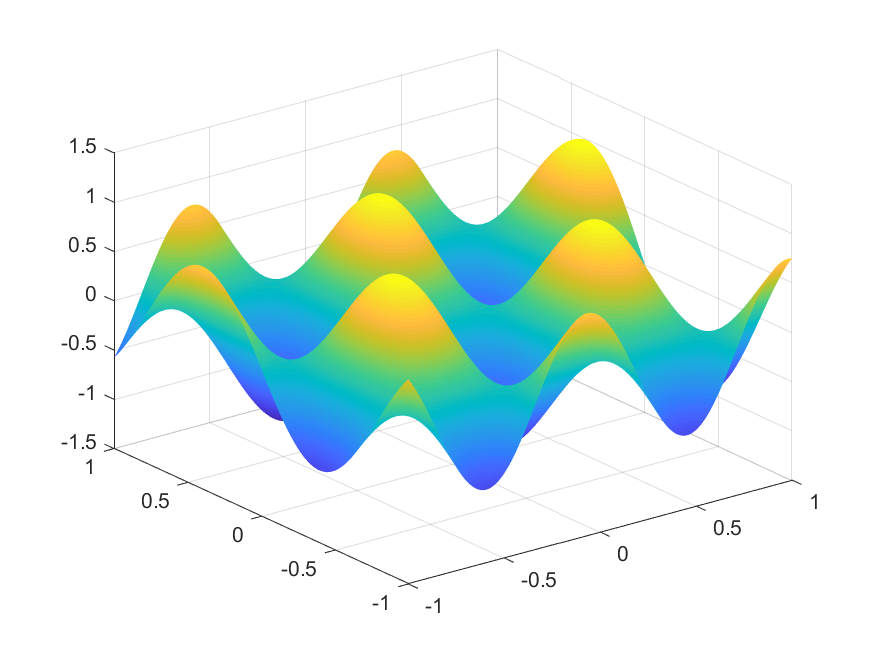
\includegraphics[width=100mm,height=60mm]{u_surface.png}
			\caption{Surface Plot of $u(x,y;t)$ at $t=2$}
		\end{figure}
		\vspace{1in}
		\begin{figure}[H]
			\centering
			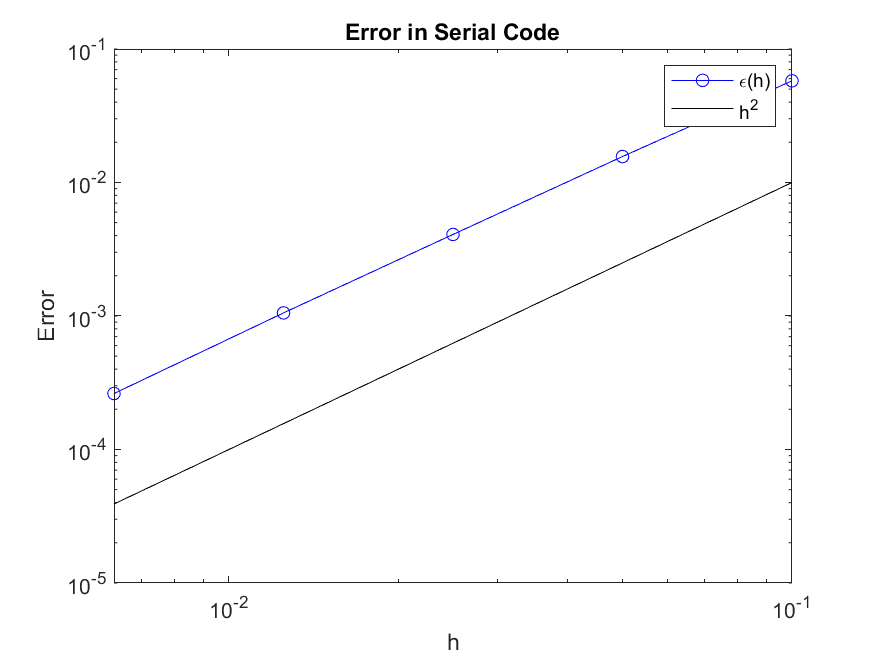
\includegraphics[width=100mm,height=60mm]{error_serial.png}
			\caption{Serial Code Error}
		\end{figure}
		\vspace{1in}
		\begin{figure}[H]
			\centering
			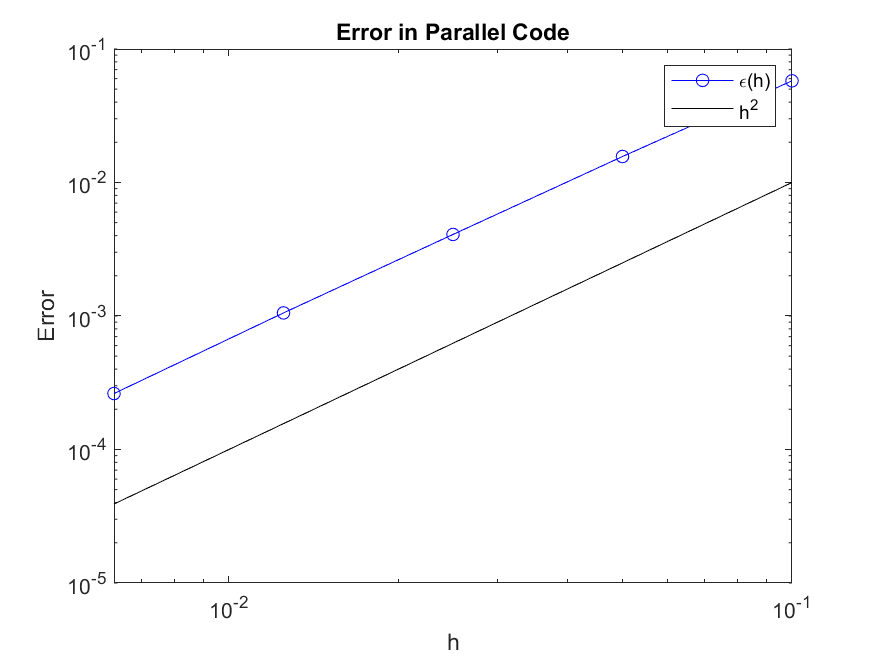
\includegraphics[width=100mm,height=60mm]{error_parallel.png}
			\caption{Strong Scaled: Parallel Code Error With 16 Cores}
		\end{figure}
		\vspace{1in}
		\begin{figure}[H]
			\centering
			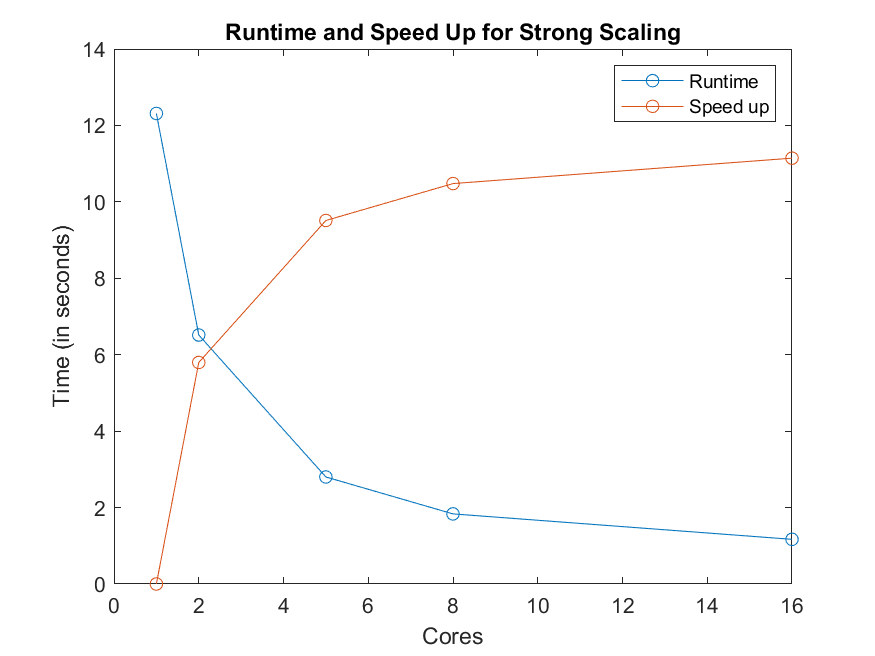
\includegraphics[width=100mm,height=60mm]{strong_time.png}
			\caption{Strong Scaled: Runtime and Speed Up}
		\end{figure}
		\vspace{1in}
			\begin{figure}[H]
			\centering
			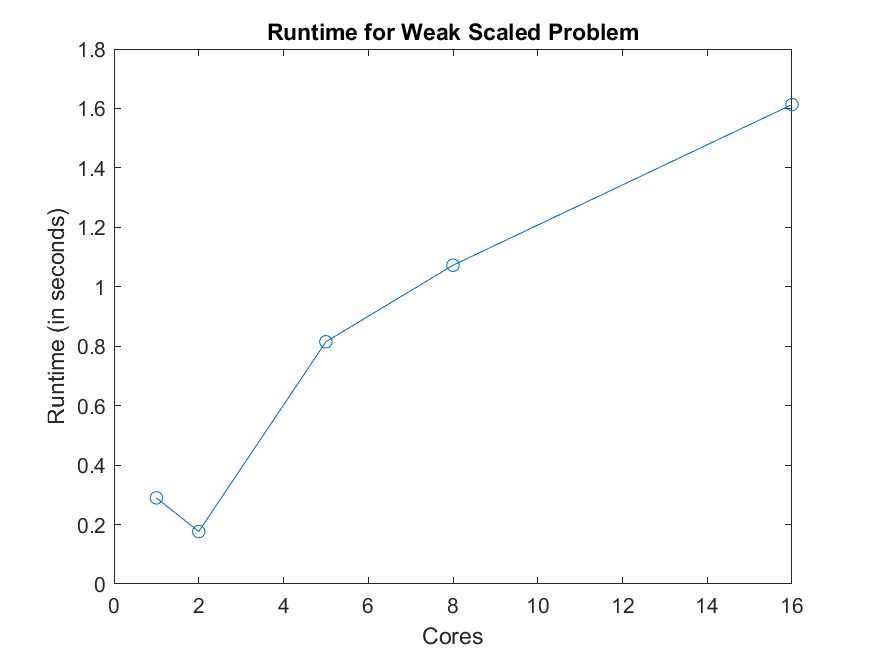
\includegraphics[width=100mm,height=60mm]{weak_time.png}
			\caption{Weak Scaled: Runtime}
		\end{figure}
		\vspace{1in}
		
        \section{Conclusion}
From the results we can conclude that there are benefits to using MPI for parallelization. We first note that the actual error in solving the IBVP stayed the same when we parallelized the code. This is evident from Figures 2 and 3 where we see that the behavior of the error is the same between the parallel and serial code. The error behaves as $O(h^2)$, which also reiterates that the Method of Lines is second order accurate. We saw benefits in speed up and efficiency in the parallel code. This is extremely evident in Figure 4 where we can clearly see that an increase in processor count decreases the runtime and increases the speedup. This is exactly what we predicted would happen prior to finding these results, due to the nature of parallel computing. 
\newline \newline
When analyzing the weak scaling we see that we did not achieve constant runtime that is expected of weak scaling. This is possibly due to a few issues, one is that the scaling factor for the grid size was not chosen correctly. The grid size was chosen to be $100n^{1/2}\times 100n^{1/2}$. A better choice for weak scaling could be $100n^{1/4}\times 100n^{1/4}$. This could possibly make the weak scaling runtimes more linear. This can be validated with more testing. 
\newline \newline
We can improve the efficiency of our MPI program by exploring more advanced MPI techniques. Our program only utilized send and receive calls, barriers and utilization of concurrent calculations. One advanced technique would be to parallelize the grid in 2D rather than 1D. This is expected to decrease the runtime further since the problem is broken up into smaller tasks. With a greater knowledge of the MPI library, we could explore more of these techniques to further utilize parallel programming.
    

\end{document}  
